\documentclass[]{article}
\usepackage{caption,subcaption,graphicx,float,url,amsmath,amssymb,amsthm,tocloft,cancel,thmtools,gensymb,braket}
\usepackage[toc,nonumberlist]{glossaries}
\usepackage{glossaries-extra}
\newcommand\numberthis{\addtocounter{equation}{1}\tag{\theequation}}

\newtheorem{thm}{Theorem}
\newtheorem{defn}[thm]{Definition}
\newtheorem{cor}[thm]{Corollary}
\newtheorem{lemma}[thm]{Lemma}
\graphicspath{{figs/}}
\widowpenalty10000
\clubpenalty10000
\setcounter{tocdepth}{1}

%opening
\title{Theoretical Minimum\\Particle Physics 1\\Basic Concepts}
\author{Simon Crase(compiler)}

\begin{document}

\maketitle

\begin{abstract}
These are my notes for Particle Physics 1 lectures from Leonard Susskind's Theoretical Minimum series.
\end{abstract}

\tableofcontents
\listoffigures

\section{Particles and Light}

Particle physics is about the question: is matter discrete? If so we will call the smallest things "particles". If matter forms a continuum, we have fields.

Which is correct? Both and neither.

First evidence for atoms came from chemistry. John Dalton looked at mass mole: each substance was an integer multiple of mass of a mole of hydrogen; it suggested that there are building blocks. We now know that mass of molecule is mass of protons, electrons (very small), and neutrons, which have nearly the same mass as protons. 
 
Figure \ref{fig:em:wave} illustrates an electromagnetic wave. We need the concepts of wavelength, $\lambda$, and period, $T$.

We have
\begin{align*}
\frac{\lambda}{T}=&c\\
f=&\frac{1}{T} \text{, so}\\
\lambda f =& c\text{. Physicists tend to measure frequency in radians per second:}\\
\omega =& 2 \pi f \text{, so}\\
\omega =& \frac{2 \pi c}{\lambda}
\end{align*}

\begin{figure}[H]
	\caption{An electromagnetic wave}\label{fig:em:wave}  
	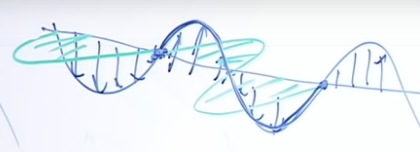
\includegraphics[width=0.9\textwidth]{Wavelength}
\end{figure}

Wave/particle duality.

A photon has energy: $E=\hslash \omega$. Energy of ray is $n \hslash \omega$

In modern usage, mass is what used to be called rest mass. $E = m c^2$ only for stationary object.

In particle physics we choose units to set $c=1$ and $\hslash=1$. 

\url{https://youtu.be/2eFvVzNF24g?t=4939}

\section{Quantum field theory}

\section{Quantum fields and particles}

\section{More quantum field theory}

\section{Energy conservation and waves}

\section{Dirac equation and Higgs particles}

\section{Angular momentum}

\section{Spin}

\section{Equations of motion of particles and fields}

\section{Field Lagrangians and path integrals}


\end{document}
